\documentclass[a4paper, 11pt]{article}
\usepackage[T1]{fontenc}
\usepackage{mathpazo}
\usepackage[hmargin=1in,vmargin=1in]{geometry}
\usepackage{amsmath,amssymb,amsthm}
\usepackage{graphicx}
\graphicspath{{manuscript/}}
\usepackage{longtable}
\usepackage{booktabs}
\usepackage{array}
\usepackage{rotating}
\usepackage{setspace}
\usepackage{subcaption}
\usepackage{xcolor}
\usepackage{authblk}
\usepackage[hyphens]{url}
\usepackage{microtype}
\usepackage{pdflscape}
\usepackage{etoolbox}
\usepackage[natbibapa]{apacite}
\usepackage[hidelinks]{hyperref}
\hyphenpenalty=10000
\setlength{\emergencystretch}{3em}
\renewcommand{\topfraction}{0.85}
\renewcommand{\textfraction}{0.10}
\renewcommand{\floatpagefraction}{0.80}
\exhyphenpenalty=10000
\interfootnotelinepenalty=10000
\widowpenalty=10000
\clubpenalty=10000
\AtBeginEnvironment{thebibliography}{%
  \interlinepenalty=10000
}

\date{October 2026}

\singlespacing

\author[1]{Timothy B. Gravelle}
\author[2]{Stuart Bagnall}
\author[2]{Antonios Katris}
\author[2]{Thomas J. Scotto}
\author[2]{Frankie Watson-Brown}
\author[3]{Jason Reifler}
\affil[1]{Wilfrid Laurier University}
\affil[2]{University of Strathclyde}
\affil[3]{University of Southampton}

\title{Nuclear Energy in the Neighbourhood?\\Examining Public Support for Small Modular Reactors in the United Kingdom}

\begin{document}

\maketitle

\begin{abstract}
\normalsize
\noindent The United Kingdom faces growing demands on its electricity grid and electricity prices as a major cost of living issue. At the same time, the UK has made a commitment to transition away from carbon-emitting sources of energy. The UK government has committed to small modular reactors (SMRs), beginning at Wylfa in Wales, yet public opinion research has only recently turned to them. Public views matter: SMRs could bring nuclear power to many more communities, and attitudes towards them are still forming. How SMRs are described and where they are sited can each prompt considerations that lead people to support or oppose them. ``Reactors'' may evoke the dangers of nuclear fission in a way that ``power stations'' do not. Siting matters in two senses: where SMRs are said to be built and how close people actually live to nuclear sites, as proximity may induce opposition by heightening perceptions of risk or support through expected economic benefits. This paper explores these issues on data from an original survey-based experiment (\textit{n} = 1,276). The experiment described SMRs as ``reactors'' or ``power stations'' developed ``in the United Kingdom'' or ``in your local area''. Support is favourable but not overly so. Calling SMRs reactors rather than power stations barely shifts support, while describing development as local lowers it modestly, consistent with ``NIMBY'' accounts. There are also regional dynamics at work, with lower support in Scotland compared to England, especially when the question posed relates to developing modular nuclear reactors in the local area. Lower support in Scotland is concentrated among supporters of independence, the constituency of a Scottish Government that, although energy is largely reserved, consents to new power stations and will not approve new nuclear projects. Support is also lower in those parts of the UK near existing nuclear sites as opposed to those further away.\\

\textit{Keywords:} Public opinion, nuclear energy, small modular reactors, framing, NIMBY, devolution, United Kingdom

\end{abstract}
\pagenumbering{roman}
\thispagestyle{empty}
\clearpage

\pagenumbering{arabic}
\section*{Introduction}
\setcounter{page}{1}
\doublespacing
Energy production and energy costs have been salient political issues in recent years in the United Kingdom. Energy costs in the UK have long been among the highest in the OECD. Geopolitical crises like the Russian invasion of Ukraine in 2022 and the 2026 US-Iran conflict have only served to drive them higher, making energy a major cost of living issue. Household subsidies for energy bills have thus been a persistent and contentious political issue for successive Conservative and Labour governments in Westminster from the Energy Price Guarantee introduced in 2022 to ongoing debates about targeted assistance with energy costs versus universal supports. Indeed, the terms ``energy debt'' and ``energy poverty'' have become part of the national conversation in the UK alongside debates about energy security.

At the same time, the UK remains legally committed to net zero emissions by 2050 under the amended Climate Change Act 2008, even if this remains politically contested. To achieve net zero, renewable and low-carbon sources of energy will have to be part of the solution. This includes nuclear energy, specifically small modular reactors (SMRs), but only if they can be built. In other countries, public opposition has proved decisive: it helped end nuclear power in Germany \citep{rudig2000,schreurs2012}, even though a majority of Germans now regard the exit as a mistake \citep{sinus2026}. SMRs are a new technology designed to be more compact and require a smaller footprint than conventional nuclear power stations, with components built offsite to allow for quicker assembly onsite. In June 2025, the UK government selected Rolls-Royce SMR as preferred bidder to build the country's first SMRs \citep{ans2025,jones2026}, and in November 2025 it named Wylfa on Anglesey as the first site, initially for three units \citep{sutton2025}. A Nuclear Regulatory Taskforce, whose call for evidence drew 30\% of its responses from wider civil society \citep{taskforce2025cfe}, has since called for a ``radical reset'' of nuclear regulation \citep{taskforce2025}, and the new national policy statement for nuclear energy (EN-7) lets developers propose sites against published criteria rather than from a fixed list \citep{desnz2025en7}. SMRs could therefore come to many more communities, and public consultation on them will largely take place in those communities. Whether the way SMRs are described, and where that engagement happens, shapes public support is therefore an important empirical question. Where they can be built also depends on devolution. Although energy is largely reserved to Westminster, Scottish Ministers decide consent for new power stations in Scotland under section 36 of the Electricity Act 1989, and the Scottish Government's policy is not to give planning consent to new nuclear projects \citep{heffron2017,scotgov2023,desnz2026anf}. In Wales, by contrast, the Wylfa SMRs are expected to be consented through the UK's infrastructure planning regime because they exceed 350 MW \citep{sutton2025}.

In this context, it is worth asking: what does the UK public think, and what factors shape individual-level support for (or conversely opposition to) SMRs? While public attitudes toward nuclear power generation are a long-standing topic of inquiry \citep{aina_poy2026,bickerstaff2008,corner2011,venables2012}, there are presently few studies examining attitudes toward SMRs \citep[but see][]{durdovic2025,jones2026,hlavacek2023,kiviluoma2025,osiolo2026}. This article explores a set of questions relating to support for SMRs in the UK. First, what is the level of public support for SMRs? Second, is support shaped by how the technology is framed, either as a power station or as a reactor? Third, does framing SMRs as a local issue versus a national one shift support? Fourth, does spatial proximity to existing nuclear sites shape support? Fifth, and more tentatively, do responses to local development differ across England, Scotland, Wales and Northern Ireland? To answer these questions, it draws on an original survey-based experiment \citep{druckman2022,mutz2011} with a national online sample of 1,276 UK adults.

To preview the main findings, SMRs enjoy broad support among the UK public. Still, framing in communication induces modest shifts in expressed levels of support: power stations receive slightly higher support than reactors, and the development of SMRs receives lower support when it is described as being in one's local area compared to when it is described as being in the UK. The results also indicate varied regional dynamics: Scots are less supportive than people in England, a gap concentrated among who would vote for Scottish independence and among supporters of the Scottish National Party. Further, Scottish support for SMRs drops particularly when they are framed as being developed in one's local area. Proximity to existing nuclear infrastructure also dampens support for SMRs.

\section*{Public Support for Nuclear Energy: Existing Research}
Because nuclear power is a relatively mature technology, attitudes toward it have received less scholarly attention in recent years than attitudes toward wind, solar, fossil fuels or electricity transmission lines \citep{carley2020}. Early studies were typically descriptive, and focused on aggregate support among the American public, showing that public support for nuclear power was divided through the 1970s and 1980s, with support decreasing in response to the Three Mile Island accident \citep{freudenburg1985, rosa1994}. Other studies focusing on the UK generally found ambivalence among the mass public, and that support for nuclear power was often tied to the need to address climate change and energy security \citep{bickerstaff2008,pidgeon2008,corner2011}. More recent work identified a drop in support for nuclear power in several countries following the Fukushima accident \citep{latre2017}, though no appreciable drop was observed in the UK \citep{jones2016}.

In terms of the factors shaping individual-level attitudes toward nuclear energy, a recent systematic review by \citet{aina_poy2026} found that perceptions of the risks and benefits associated with nuclear energy were the most consistent factors associated with support or opposition. This is consistent with earlier research examining the social construction of nuclear risk \citep{gamson1989} and risk perceptions \citep{pidgeon2008,greenberg2009,degroot2013,slovic2000,vanderpligt1986}. Other attitudinal factors that have been found to shape attitudes toward nuclear energy include ideological (or left--right) orientations, with those on the right expressing greater support \citep{besley2014,franchino2014,mcbeth2023,sonnberger2021}. Trust in government institutions, regulatory authorities, and power companies themselves is also positively associated with support for nuclear power \citep{konisky2020,mcbeth2023}. Importantly, in spite of the low carbon emissions associated with generating nuclear energy, concern with climate change has often been found to be negatively associated with support for nuclear energy \citep{corner2011,konisky2020,sonnberger2021}. Explanations for this seemingly paradoxical yet consistent finding include the lack of knowledge about nuclear energy's low carbon footprint among the public \citep{bickerstaff2008} and a preference for other renewable sources of energy -- i.e., solar, wind, and hydroelectricity -- over nuclear among those expressing high levels of climate concern \citep{pidgeon2008}.

As for demographic factors associated with support for nuclear energy, the most noteworthy result is that women consistently express lower support than men \citep{aina_baici_poy2026,cale2015,corner2011,greenberg2009,kiviluoma2025,konisky2020,sonnberger2021,venables2012}. The principal explanation for this finding is that women tend to express higher perceptions of risk related to nuclear energy compared to men \citep{degroot2013,slovic2000}.

Existing research has also examined the effect of proximity to nuclear sites on support, though the available evidence is not definitive with respect to either a ``NIMBY'' (not in my backyard) or an ``inverse-NIMBY'' dynamic. In some contexts, particularly where proximity raises familiarity with nuclear energy and perceptions of local economic benefits, greater proximity is associated with higher support \citep{greenberg2009,mcbeth2023,vanderpligt1986}. Other work finds no such proximity effect in multivariate analyses that include a range of attitudinal variables \citep{aina_baici_poy2026,cale2015,konisky2020}. Such null findings may reflect the fact that individuals often lack accurate knowledge of their actual proximity to nuclear sites \citep{lyons2020}. A further set of studies, which either experimentally manipulate the proximity of a proposed nuclear facility or ask about near and distant proposed sites in sequence, uncovers a NIMBY dynamic: more distant sites are preferred over more proximate ones \citep{biten2026,durdovic2025,hlavacek2023,jones2026,kiviluoma2025,seo2026}.

Because SMRs are a relatively new technology, there are currently few studies of attitudes toward them. To date, research focusing on the UK and continental Europe has found that knowledge about SMRs remains low, and support for their construction is tepid \citep{durdovic2025,jones2026,kiviluoma2025}. Research by Hlavacek and colleagues (\citeyear{hlavacek2023}) reconfirms many of the central results of the literature on attitudes toward nuclear energy: trust in government is positively associated with support, climate concern is negatively associated, and support is lower among women. Further, support is lower when a proposed SMR is described as nearby as opposed to further away. Experiments on new nuclear plants more generally point the same way: support falls when a proposed fusion or next-generation fission plant, including small modular designs, is within 20 km rather than 80 km or more of respondents' homes in six European countries including the UK \citep{biten2026}, and when a proposed US plant is made locally salient \citep{seo2026}.

While existing research has identified several individual-level determinants of attitudes towards nuclear energy, far less attention has been paid to how these attitudes vary across subnational political and institutional contexts. The distinction matters in the United Kingdom. Energy policy is largely reserved to Westminster for Great Britain but devolved in Northern Ireland, which also belongs to the all-island Single Electricity Market with Ireland rather than the Great Britain market. The four nations also differ in their political institutions, energy-policy priorities, administrative systems and histories of nuclear development. Scotland has hosted nuclear stations at Hunterston, Torness, Chapelcross and Dounreay, yet its government will not consent to new ones \citep{heffron2017, scotgov2023,desnz2026anf}. Wales will host the first SMRs, at Wylfa, with its government's support \citep{sutton2025}. Northern Ireland has never had a nuclear power station. Such differences may shape how citizens weigh the benefits and risks of nuclear infrastructure, particularly when development is framed as affecting their own community rather than the country as a whole. The effect of local framing therefore need not be uniform across the UK. Alongside the overall effects of terminology and local siting, we explore whether responses to local nuclear development differ across England, Scotland, Wales and Northern Ireland. This allows us to assess not only whether terminology and the geographic scale of proposed development shape public support, but also whether the effect of local framing varies across distinct political and institutional contexts.

\section*{Theoretical Expectations}

Analysts of public opinion have long recognised that attitudes toward particular objects are shaped by how they are depicted and discussed -- that is, how they are framed. In general terms, frames are the ways in which communication about an object (whether a policy, a technology, a social issue, or anything else) selects or emphasises particular aspects related to that object, rendering these aspects more salient \citep{entman1993}. Framing effects are shifts in individual-level attitudes that are the consequence of communications that activate (or assign greater importance to) different considerations \citep{chong2007,druckman2001,nelson1997}. Specifically in survey settings, responses are shaped by the frames employed in the questions asked \citep{zaller1992}.

Frames are certainly relevant to energy issues. For example, Clarke and colleagues (\citeyear{clarke2015}) find that \emph{fracking} is seen as having greater risks, more negative consequences, and has less public support than \emph{shale oil and gas development}. \citet{stokes2017} find that job benefit and air pollution reduction frames increase support for renewable energy. In the case of nuclear energy, frames are equally relevant. There are long-standing frames present in the news media. Seminal work by \citet{gamson1989} identified a set of frames employed in media coverage of nuclear power, the most prevalent being technological progress and what they termed ``runaway'' -- the notion that nuclear energy had outrun the ability of humankind to control it, and clearly intended to evoke an uncontrolled (or runaway) nuclear chain reaction. These progress and risk frames have been studied from other angles. Using a word association task and the stimulus term ``nuclear power,'' Slovic and colleagues (\citeyear{slovic2000}) find that responses having negative associations outweighed positive ones. Outside of references to nuclear warfare, the most common negative associations related to nuclear waste and nuclear accidents or meltdowns \citep{slovic2000}. Further, Bolsen and colleagues (\citeyear{bolsen2014}) find that a health risk frame decreases support for nuclear power. Qualitative evidence indicates that such risks are an important consideration in how citizens think about nuclear energy \citep{bickerstaff2008}.

We build on previous work by testing alternative terms: small modular nuclear \emph{reactors} and small modular nuclear \emph{power stations}. Just as \emph{fracking} carries more negative connotations and is more closely linked to environmental and health risks than \emph{shale oil and gas development} \citep{clarke2015}, so too does \emph{reactor} relative to the more benign \emph{power station}. The term \emph{reactor} evokes the risks associated with nuclear fission and uncontrolled chain reactions, whereas a \emph{power station} is a relatively mundane feature of the built environment. Our first hypothesis is thus:

$H_1$: Support for SMRs will be lower when they are described as small modular nuclear \emph{reactors} than when they are described as small modular nuclear \emph{power stations}.

Mass public opinion is often shaped by features of the built environment. Indeed, a large body of literature has examined how public support for (or opposition to) different forms of energy exploration, generation, and transmission is shaped by \emph{proximity} to energy sites \citep[see, e.g.,][]{aldrich2013,boudet2018,clarke2016,evensen2016,gravelle2015,konisky2020,latre2017,mueller2019,mueller2017}. The focus on proximity effects is well motivated: individuals more readily draw on cues from what is \emph{near} in forming their opinions and attitudes than what is \emph{far away}. Psychological research on construal level theory \citep{fujita2006,henderson2006,trope2007,trope_liberman2010} posits that the mental representations of events and objects that are proximate (in either space or time) are concrete and detailed; those that are distant are abstract.

Still, existing research is equivocal on the question of whether and how proximity matters to mass public attitudes toward energy issues. On the one hand, proximity may act to heighten perceptions of the risks associated with various technologies \citep{boudet2018,venables2012}. On the other hand, proximity may serve to highlight localised benefits, such as jobs tied to energy generation or the construction of energy infrastructure \citep{aldrich2013,gravelle2015}. For example, \citet{gravelle2015} find that proximity to the proposed route of the Keystone XL pipeline increases support, principally among self-described liberals (while conservatives are consistently in favour whether near or far from the pipeline); this finding is largely confirmed by Clarke and colleagues (\citeyear{clarke2016}). Conversely, Mueller and colleagues (\citeyear{mueller2017}) and \citet{mueller2019} find that proximity to electricity grid projects reduces support for grid expansion. Alcorn and colleagues (\citeyear{alcorn2017}) find no consistent effect of proximity to fracking sites on support, a finding in line with Konisky and colleagues (\citeyear{konisky2020}) who examine a range of energy generation and transmission projects.

Studies of attitudes toward nuclear energy exhibit the same sort of disparate findings as other sources of energy. While \citet{greenberg2009}, McBeth and colleagues (\citeyear{mcbeth2023}) and van der Pligt and colleagues (\citeyear{vanderpligt1986}) find that residents near a nuclear site had more positive attitudes toward nuclear energy than those further away, a cross-national study by Latré and colleagues (\citeyear{latre2017}) finds that the Fukushima nuclear accident induced a negative shift in public attitudes toward nuclear energy, with larger negative shifts in countries closer to Japan. By contrast, Aina and colleagues (\citeyear{aina_baici_poy2026}), \citet{cale2015}, and Konisky and colleagues (\citeyear{konisky2020}) find no effect of proximity to nuclear sites on attitudes toward nuclear energy. Two factors may underlie such varied results. The first is that proximity/distance is operationalised by different authors in different ways. In many studies, ``near'' is operationalised as residents within a given radius of a nuclear site (ranging from 1 to 50 miles); few studies use actual geodetic distances. Second, the localised risks and economic benefits of particular nuclear sites may vary across local contexts, thus shaping the balance of local considerations relating to opposition or support.

Most existing research on proximity effects and support for nuclear energy relates to existing nuclear sites. Neither the siting of nuclear facilities nor where people live is random, however. An alternative research strategy is to experimentally manipulate the salience of nuclear energy in one's milieu. Experimental research that has done so has produced results that stand in contrast to the equivocal character of findings of observational survey research. In survey-based experiments, Biten Butorac and colleagues (\citeyear{biten2026}) and \citet{seo2026} both find that describing a proposed nuclear plant as nearby as opposed to further away reduces support for its construction. Thus citizens, most of whom have little previous direct contact with nuclear energy and for whom it is literally a distant consideration, are less favourable toward building new nuclear energy infrastructure nearby. These results are further supported by observational research showing greater support for SMRs at a more distant site when respondents are also asked about support for construction nearby \citep{durdovic2025,hlavacek2023,jones2026,kiviluoma2025}.

Considering the sum total of existing research findings, we follow recent research and advance a directional hypothesis indicating that mass publics exhibit less support for SMRs when they are described as being nearby (as opposed to further away).

$H_2$: Support for SMRs will be lower when they are described as being in one's local area compared to being in the United Kingdom.

At the same time, we consider it appropriate to advance a non-directional (two-tailed) hypothesis relating to the association between (actual) distance to the nearest nuclear site and support for SMRs.

$H_3$: Spatial distance to a nuclear site will be associated with support for SMRs.

Finally, because the UK's four nations differ in their institutions and histories of nuclear development, we pose an exploratory research question rather than a directional hypothesis.

$\mathit{RQ}_1$: Does the effect of the local frame differ across the UK's four nations?

\section*{Data and Methods}

To test these theoretical expectations, we undertake a survey-based experiment \citep{druckman2022,mutz2011}. Our experiment was administered to a sample of 1,276 adults residing in the United Kingdom. Participants were members of the Vox Pop Labs online panel. As a civic engagement and digital technology firm, Vox Pop Labs recruits into its online panels principally from users of its voting advice application, \emph{Vote Compass}, who volunteer to participate in future research studies. Survey data collection took place from 7 October to 11 November 2025. The study received ethics approval from the University Ethics Committee at the University of Strathclyde.

Though our online panel participants comprise a non-probability sample, we argue that such a sample is fit for purpose given the goals of our research \citep[cf.][]{baker2013}. One of our principal aims is to assess the effects of our experimental manipulations, and several studies have concluded that online non-probability samples yield experimental treatment effect estimates that do not differ substantively from those obtained from probability samples \citep{coppock2018,krupnikov2014,mullinix2015}.

We nevertheless approach the task of drawing inferences from non-probability survey samples as one needing careful consideration. We thus draw on model-based approaches to weighting non-probability samples that have been advanced in the survey methodology literature. Specifically, we use the quasi-randomization method to estimate pseudo-inclusion probabilities for observations from a non-probability sample when a probability-based reference survey is available \citep{elliott2009,elliott_valliant2017,lee2009}. In brief, probabilities of selection for observations from a non-probability sample can be estimated via logistic regression by pooling the data with an external probability-based survey (termed a reference survey) that contains the same set of covariates as the non-probability sample. We use the 2022--2024 Annual Population Survey (conducted by the Office for National Statistics) as the probability-based reference survey for this purpose. The initial weights obtained by taking the inverse of these estimated probabilities of selection for our Vox Pop Labs panel members are further adjusted (raked) to align the sample with the demographic and political profile of the United Kingdom general public. Each experimental condition (discussed below) is weighted separately on sex, age, educational attainment, country of birth (the UK or abroad), region, and recalled vote from the 2024 general election. This set of weighting procedures allows us to make estimates of treatment effects among the UK public.

The key elements of our survey design are as follows (we reproduce the full survey instrument in the online replication materials). The survey began by asking participants about their attention to government and public affairs, their opinion about the most important issue facing the UK, and their knowledge and attitudes about electricity issues in the UK. Building on existing research showing that climate attitudes, trust in government, and trust in electricity companies all shape attitudes toward energy infrastructure \citep{aina_poy2026,konisky2020}, the survey then asked participants a series of questions on these topics.

Participants were then presented with a brief description of SMRs, and then asked a question on their level of support for them that incorporated our two experimental manipulations. These manipulations were randomised independently -- i.e., in a $2 \times 2$ factorial design. Based on our expectations relating to the effect of ``power station'' versus ``reactor'' language, the first experimental manipulation randomised the use of the terms small modular nuclear reactors (SMNRs) and small modular nuclear power stations (SMNPs). Both terms include ``nuclear'' because public familiarity with SMRs is low \citep{durdovic2025,jones2026}, and the shorter label might not signal a nuclear technology. Motivated by our NIMBY expectations, the second experimental manipulation randomised whether SMRs were described as being in ``the United Kingdom'' or ``your local area.'' The overall design of the experimental stimulus is presented below in Figure~\ref{fig:stimulus}, with the bold text inside square brackets to highlight which aspects of the stimulus were randomised. Following this experimental manipulation, participants were asked to rate their support for the development of SMNRs (or SMNPs) on a five-point response scale from strongly support (scored +0.5) to strongly oppose (scored $-$0.5), with ``Not sure'' responses (56 in total) recoded to the middle ``Neither support nor oppose'' response.\footnote{This recoding of the dependent variable does not alter our substantive conclusions. Tables A3--A4 in the online appendix provide the results for all models with non-responses on dependent variable removed from the analyses.}

\begin{figure}[!htbp]
\centering
\fbox{\begin{minipage}{0.9\linewidth}
\vspace{4pt}
\textbf{[Small Modular Nuclear Reactors (SMNRs)] [Small Modular Nuclear Power Stations (SMNPs)]} are a new type of nuclear \textbf{[reactor] [power station]} that can be built in factories and assembled on site. They take up less space than traditional nuclear \textbf{[reactors] [power stations]}, and are designed to provide low-carbon electricity.

\medskip
To what extent do you support or oppose the development of \textbf{[SMNRs] [SMNPs]} in \textbf{[the United Kingdom] [your local area]}?

\medskip
\hspace*{2em}Strongly support\\
\hspace*{2em}Somewhat support\\
\hspace*{2em}Neither support nor oppose\\
\hspace*{2em}Somewhat oppose\\
\hspace*{2em}Strongly oppose\\
\hspace*{2em}Not sure
\vspace{4pt}
\end{minipage}}
\caption{Experimental stimulus}
\label{fig:stimulus}
\end{figure}

After the experimentally manipulated question on SMRs, participants were asked questions about political party identification, voting intentions in a future general election, recalled vote from the 2024 general election, left--right ideological orientations, as well as their personal demographic characteristics.

Testing our theoretical expectation about proximity to existing nuclear energy infrastructure requires us to place our participants on the map, and then calculate their proximity to -- or conversely, distance from -- existing nuclear energy sites, both active and decommissioned. To do so, we assign National Grid coordinates to the survey participants using their self-reported postcodes in conjunction with data products from the Office for National Statistics (the National Statistics Postcode Lookup dataset) and the Ordnance Survey (the Code-Point with Polygons shapefile). For nuclear energy infrastructure, we draw on the site location data made available as part of the Digest of UK Energy Statistics (DUKES) annual reports for 2001 to 2024, now published by the UK Department for Energy Security and Net Zero (\url{https://www.gov.uk/government/collections/digest-of-uk-energy-statistics-dukes}). This allows us to collate a list of nuclear energy sites. Performing a spatial join (point to point) between these two datasets provides us with the distance (in kilometres) to the nearest nuclear site for each participant. The resulting distance values range between 1.9 and 523.0 kilometres with a mean value of 83.2 kilometres. As a placebo, we also calculate each participant's distance to the nearest power station of any type (mean 7.8 kilometres).

To evaluate our theoretical expectations, we estimate a set of linear regression models in a Bayesian statistical framework \citep{gill2024,kaplan2023} with 5 chains and 10,000 post-warmup iterations for each chain using the \emph{brms} package \citep{burkner2017} version 2.23.0 in R version 4.6.0 as a front-end to estimation in \emph{Stan}. Our focus is on the main effects of our two experimental manipulations along with the effect of proximity to nuclear energy infrastructure. We report below the posterior means for our coefficients ($\beta$), the posterior standard deviations (\emph{SD}) as measures of uncertainty, as well as the equal-tailed 95\% credible intervals (CrI) from these Bayesian models. We also report the posterior probabilities ($P(\beta)$) for specific effects where these are relevant.

Our models include a set of demographic covariates: country (that is, England, Wales, Scotland, and Northern Ireland), sex, age, and educational attainment. We also follow existing research on attitudes toward energy generation and transmission infrastructure \citep{aina_poy2026,konisky2020} and include model specifications that include a set of attitudinal covariates. These are: left--right ideological orientation, following news about electricity issues (as a measure of issue awareness), beliefs about the need for the UK to produce more electricity, the need for the UK to become self-sufficient in electricity, the need to keep the price of electricity in the UK low, and composite measures (created from a confirmatory factor analysis model) of climate concern, trust in government, and trust in electricity companies. Age and distance to the nearest nuclear site are logged and centred at their weighted means, and all other non-categorical covariates, including the factor scores, are rescaled to run from 0 to 1 and centred at their weighted means. Missing and ``don't know'' responses on covariates are few, except for left--right position (44 respondents); they are set to the scale midpoint for attitudinal items and to the lowest category for education and attention to electricity news. We include these covariates for their domain relevance, and to improve the precision of the estimates of experimental effects (\citealp[pp.~96--105]{gerber2012}; \citealp{lin2013}). Table A1 in the online appendix reports a model with only the experimental factors, distance and demographic covariates (Model 0).

\section*{Results}

We find that public support for SMRs in the UK is generally favourable. Across our experimental conditions, and without adjusting for covariates, mean support ranges between 0.193 and 0.282 on our five-category ($-$0.5 to +0.5) response scale.

Turning to the effects of our experimental manipulations, the results from Model 1 indicate that describing SMRs as small modular nuclear \emph{reactors} (as opposed to small modular nuclear \emph{power stations}) yields slightly lower support ($\beta = -0.026$, \emph{SD} = 0.014, CrI = $[-0.050, 0.001]$, $P(\beta < 0) = 0.972$). Models 2 and 3 yield very similar results (see Figure~\ref{fig:coefplot}). The effect is small: the credible interval excludes a penalty larger than 0.05 on the scale.\footnote{Without the attitudinal covariates, the reactor estimate is $-0.047$, \emph{SD} = 0.015, (CrI = $[-0.076, -0.017]$; see Model 0 in Table A1 in the online appendix. Because assignment was random, adjustment should affect precision rather than the expected effect; the difference reflects chance imbalance between the reactor and power-station experimental arms in three strong predictors of support: beliefs that the UK needs more electricity, attention to electricity news, and left--right ideological position. We therefore treat the adjusted estimate as our best estimate of the terminology effect.} In substantive terms, public support for SMRs remains favourable whether the technology is described as power stations or reactors, with only a slight negative shift in the case of the latter term. This is further shown in predicted scores for the constituent parts of the UK in Figure~\ref{fig:pred-frame}.\footnote{These predicted scores are calculated from Model 3 by setting all continuous covariates to their means, sex to female, and the local--UK experimental manipulation to the \emph{United Kingdom} level.} In England, the predicted support for power stations is 0.237, while it is 0.211 for reactors. Predicted support in Scotland is slightly lower, with 0.192 for power stations and 0.166 for reactors. Predicted support in Wales is 0.251 for power stations and 0.225 for reactors, while it is 0.270 for power stations and 0.244 for reactors in Northern Ireland.

\begin{figure}
    \centering
    \includegraphics[width=\linewidth]{Fig 2-Coefficient plot-2026 10 26.png}
    \caption{Coefficient plot: experimental effects and covariates. Horizontal lines are 95\% credible intervals.}
    \label{fig:coefplot}
\end{figure}

\begin{figure}
    \centering
    \includegraphics[width=\linewidth]{Fig 3-Effect plot-Country x reactor 2026 10 26.png}
    \caption{Predicted support for SMRs by power station--reactor framing and country (Model 3). Error bars are 83\% credible intervals; non-overlap approximates a difference at the 95\% level.}
    \label{fig:pred-frame}
\end{figure}

The results from Models 1--3 further indicate that asking about support for modular nuclear energy generation in one's \emph{local area} (as opposed to in the \emph{United Kingdom}) softens support. Model 1 estimates the main effect of the local area--UK experimental manipulation, and this shows a negative effect for the local area framing ($\beta = -0.041$, \emph{SD} = 0.014, CrI = $[-0.069, -0.013]$). While statistically robust, and congruent with previous research \citep{biten2026,seo2026}, the magnitude of this effect again indicates that mass opinion in the UK overall remains broadly favourable toward modular nuclear energy generation, regardless of whether it is presented as in the UK (and potentially some considerable distance away) or in one's local area.

Support is also lower in Scotland than in England (Model 1: $\beta = -0.114$, \emph{SD} = 0.025, CrI = $[-0.162, -0.065]$), while the estimates for Wales and Northern Ireland are close to zero. Yet Model 1 tests only the main effect of the local area framing. Models 2 and 3 relax this assumption by interacting the local area--UK manipulation with country, thereby testing for heterogeneous treatment effects across the constituent parts of the UK. Model 2 includes interaction terms for Scotland, Wales, and Northern Ireland, contrasting the effect of the local area framing in these parts of the UK with its effect in England. The results indicate that the local area frame has a substantially larger negative effect in Scotland compared to England. While the lower-order term (indicating the effect in England) remains negative ($\beta = -0.030$, \emph{SD} = 0.015, CrI = $[-0.058, -0.001]$, $P(\beta < 0) = 0.979$), the higher-order Scotland $\times$ local area interaction term is large and negative ($\beta = -0.142$, \emph{SD} = 0.046, CrI = $[-0.232, -0.051]$). The Bayes factor comparing Model 2 and Model 1 is 10.125, providing strong evidence to conclude that Model 2 ought to be preferred over Model 1.

Given the near-zero interaction terms for Wales and Northern Ireland, Model 3 tests a different Model specification with only a Scotland $\times$ local area higher-order interaction term, imposing a common slope for the local area effect in England, Wales, and Northern Ireland while allowing the slope for Scotland to vary. This model specification yields nearly identical results: the lower order term is again negative ($\beta = -0.031$, \emph{SD} = 0.014, CrI = $[-0.059, -0.003]$, $P(\beta < 0) = 0.985$) while the Scotland $\times$ local area higher-order interaction term is again strongly negative ($\beta = -0.141$, \emph{SD} = 0.046, CrI = $[-0.230, -0.051]$, $P(\beta < 0) = 0.999$, $P(\text{combined} < 0) > 0.999$). The Bayes factor comparing Model 3 and Model 1 is 34.751, again providing strong evidence that Model 3 outperforms Model 1. The markedly different response of Scots to the local area frame is apparent in the predicted scores shown in Figure~\ref{fig:pred-local}.\footnote{These predicted scores are similarly calculated by setting all continuous covariates to their means, sex to female, and the power station--reactor experimental manipulation to the \emph{power station} level.} The predicted support for modular nuclear energy in England is 0.237 when it is described as being in the UK and 0.206 when it is described as being in one's local area. In Wales, predicted support is at similar levels: 0.251 in the UK and 0.220 in one's local area. The same holds in Northern Ireland where predicted support for modular nuclear energy is 0.270 in the UK and 0.239 in one's local area. By contrast, predicted support in Scotland is 0.192 when it is described as being in the UK; predicted support drops to 0.021 when it is described as being in one's local area. This result may reflect the distinct politics of nuclear siting in Scotland, which was seen by Scottish nationalists as imposed by Westminster \citep{ross2024}.

\begin{figure}
    \centering
    \includegraphics[width=\linewidth]{Fig 4-Effect plot-Country x local 2026 10 26.png}
    \caption{Predicted support for modular nuclear energy by local--UK framing and country (Model 3). Error bars are 83\% credible intervals; non-overlap approximates a difference at the 95\% level.}
    \label{fig:pred-local}
\end{figure}

While the local area--UK experimental manipulation involved an attempt to consider nuclear energy generation as a proximate (as opposed to a distant) consideration, actual spatial proximity to existing nuclear energy sites also matters. In Model 3, logged distance to an active or decommissioned nuclear site exhibits a modest positive association with support for modular nuclear energy generation ($\beta = 0.026$, \emph{SD} = 0.011, CrI = $[0.005, 0.047]$); the results from Models 1 and 2 are very similar. Substantively, this association indicates that support for modular nuclear energy generation increases with greater distance from existing nuclear energy sites. Conversely, closer proximity to existing nuclear energy sites is associated with reduced support -- implying a NIMBY dynamic. Again, generating predicted scores (in this case, focusing on England and Scotland, for participants in the \emph{local area} and \emph{power station} conditions) illustrates the substantive importance of proximity to nuclear sites on support (see Figure~\ref{fig:pred-distance}).\footnote{These predicted scores are again calculated by setting all continuous covariates to their means, sex to female, the power station--reactor experimental manipulation to the \emph{power station} level, and the local--UK experimental manipulation set in this instance to the \emph{local} level.}. In England, predicted support is 0.155 at a distance of 10 kilometres, increasing to 0.197 at 50 kilometres, 0.215 at 100 kilometres and 0.233 at 200 kilometres. By contrast, predicted support in Scotland is $-$0.031 at a distance of 10 kilometres, 0.011 at 50 kilometres, 0.029 at 100 kilometres and 0.047 at 200 kilometres. It is worth highlighting that this association is robust in the face of several covariates, including demographic characteristics, left-right ideology, climate attitudes, trust in electricity companies, and beliefs about electricity generation.

\begin{figure}
    \centering
    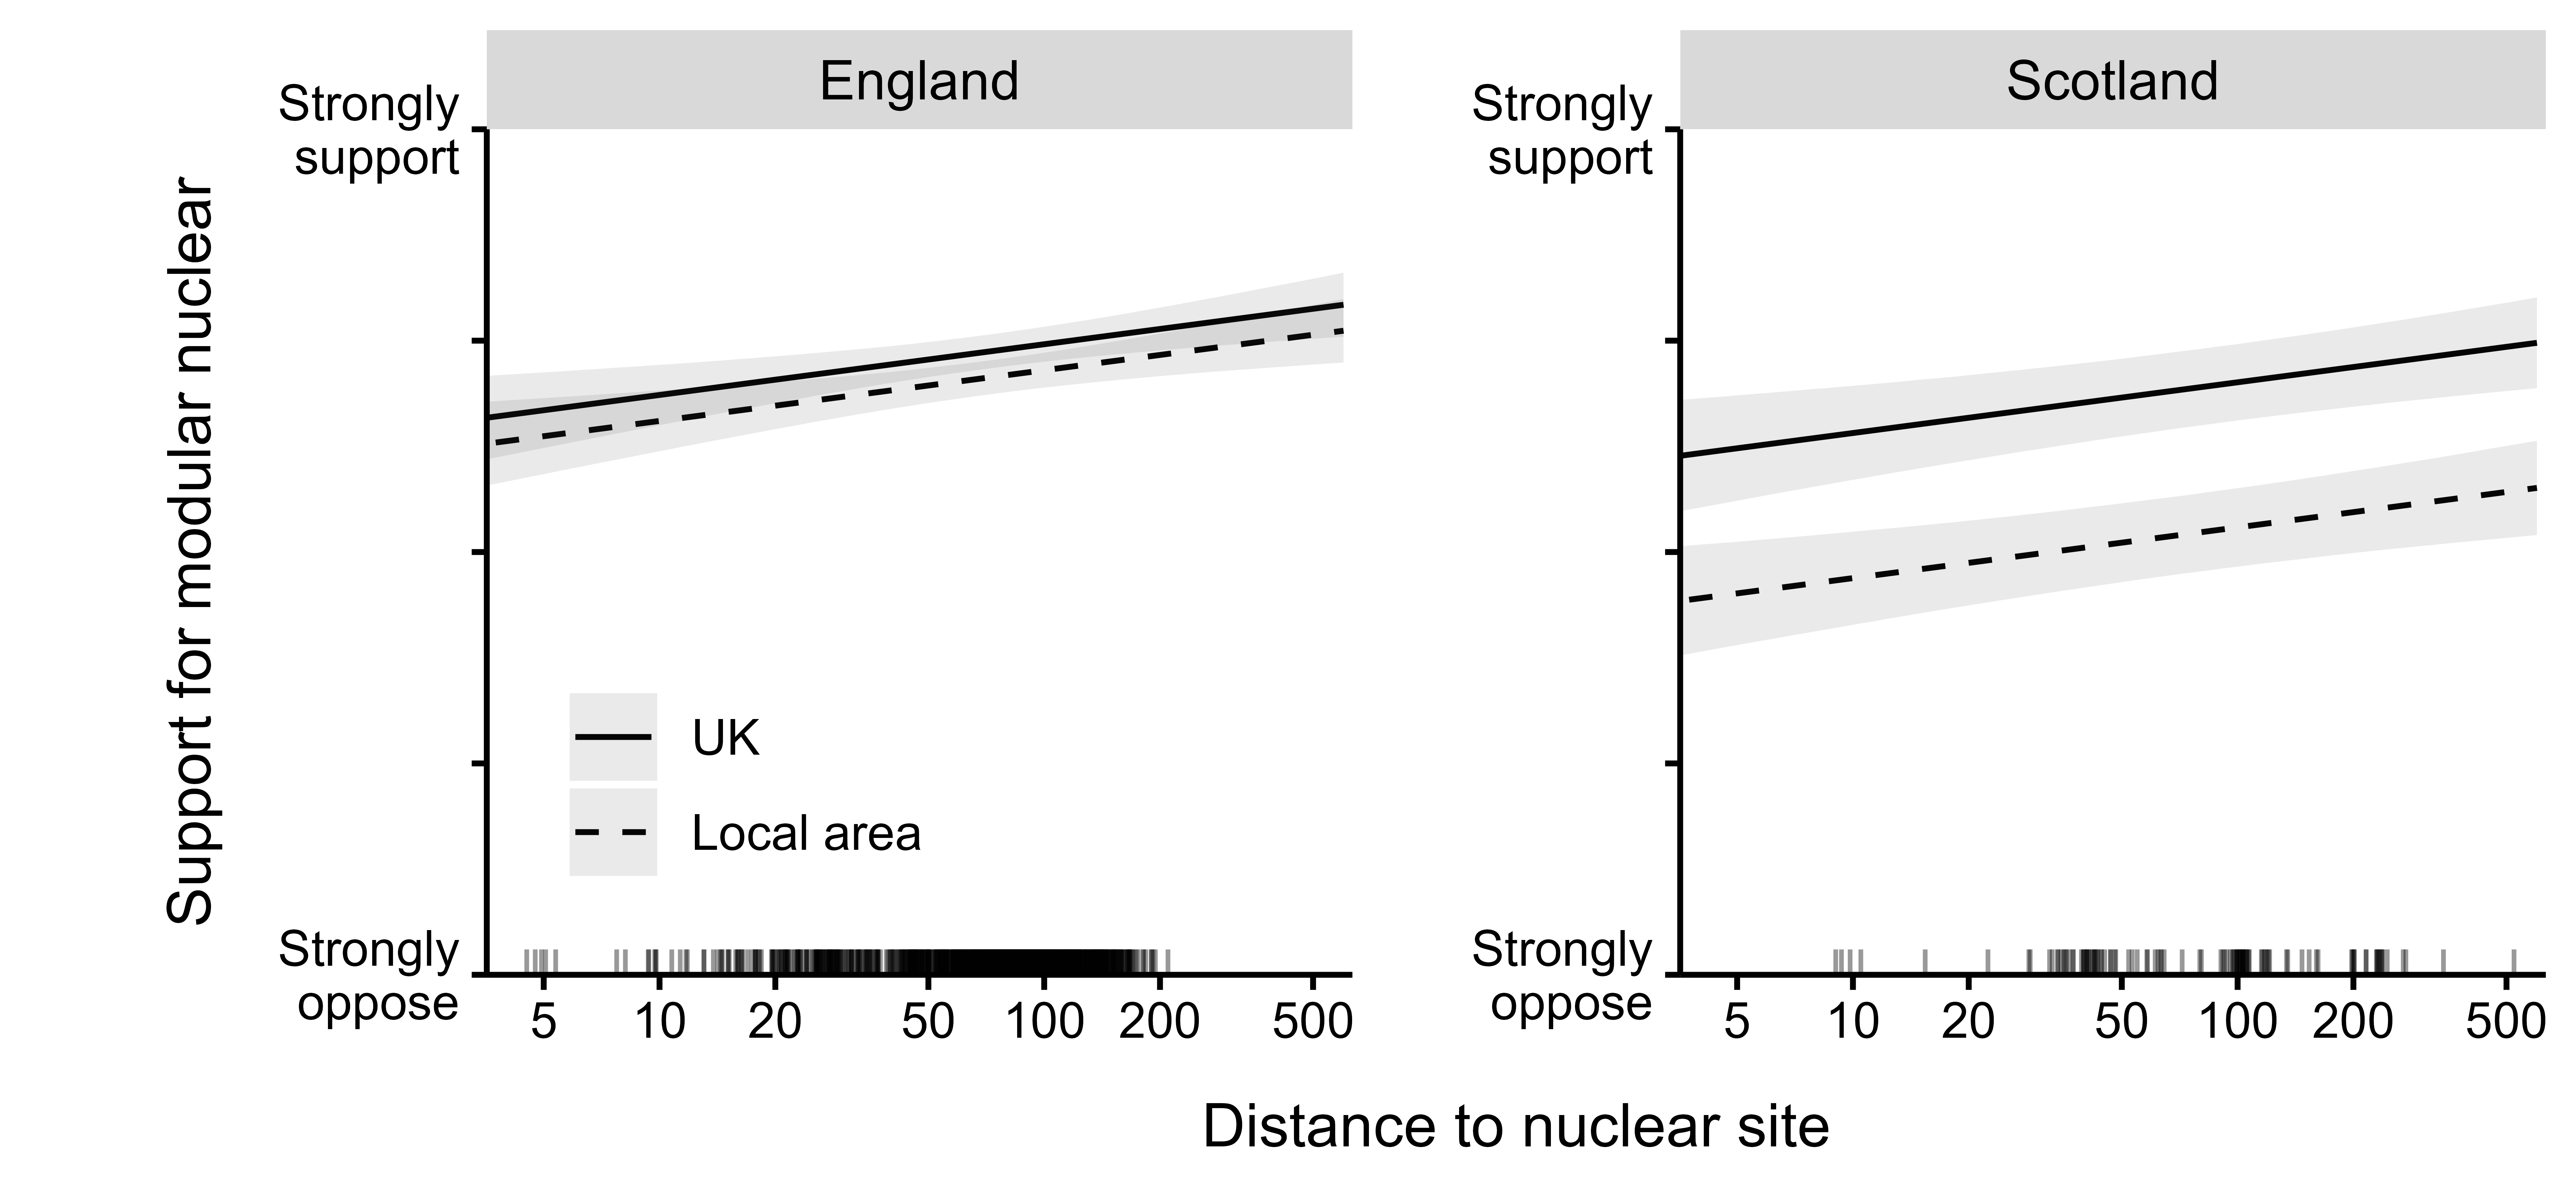
\includegraphics[width=\linewidth]{Fig 5-Effect plot-Country frame dist 2026 10 26.png}
    \caption{Predicted support for SMRs by distance to nuclear site, England and Scotland (Model 3). Shaded bands are 83\% credible intervals; non-overlap approximates a difference at the 95\% level.}
    \label{fig:pred-distance}
\end{figure}

To look deeper into the sources of Scotland's lower support for SMRs, we use respondents' voting in a hypothetical referendum on Scottish independence as well as their recalled vote in the 2024 general election and their party identification in a set of additional regression models (Models 5--7, reported in Table A2 in the online appendix).\footnote{These questions were asked after the experimental stimulus. It is unlikely that the description of SMRs altered respondents' constitutional preferences, recalled vote or party identification.} Scots who would vote for independence are markedly less supportive of SMRs than people in England ($\beta = -0.254$, \emph{SD} = 0.036, CrI = $[-0.325, -0.182]$), whereas Scots who would vote against independence (or who would not vote, or are unsure) are indistinguishable from them ($\beta = -0.004$, \emph{SD} = 0.033, CrI = $[-0.068, 0.060]$). A similar pattern appears when looking at 2024 SNP voters. Compared to those in England, SNP voters express substantially less support for SMRs ($\beta = -0.237$, \emph{SD} = 0.043, CrI = $[-0.322, -0.152]$); other Scots are only slightly lower in their levels of support ($\beta = -0.057$, \emph{SD} = 0.029, CrI = $[-0.113, -0.002]$). Looking at party identification instead of voting behaviour reveals the same thing. Scots who identify with the SNP express less support for SMRs than those in England ($\beta = -0.218$, \emph{SD} = 0.048, CrI = $[-0.312, -0.123]$), whereas other Scots are only slightly lower in their levels of support ($\beta = -0.077$, \emph{SD} = 0.028, CrI = $[-0.131, -0.024]$). Such lower support for SMRs among supporters of Scottish independence and the SNP is consistent with narrative accounts of the pro-independence and anti-nuclear movements in Scotland, which have long been intertwined \citep{brown2017,ross2024}.

Considering some of the observational covariates, both following news about electricity and beliefs that the UK needs to produce more electricity in the future are positively associated with support for SMRs. Support is therefore linked to both issue salience as well as a recognition that electricity supply must expand. Trust in electricity companies and suppliers is also positively associated with support for SMRs, a result that aligns with Konisky and colleagues (\citeyear{konisky2020}). Concern over climate change is negatively associated with support for SMRs, a finding that accords with the findings of Corner and colleagues (\citeyear{corner2011}), Konisky and colleagues (\citeyear{konisky2020}), and Sonnberger and colleagues (\citeyear{sonnberger2021}). This holds despite the lower CO\textsubscript{2} emissions associated with nuclear energy compared to fossil fuels. Also, those on the political right are more supportive of SMRs, a finding congruent with \citet{franchino2014}, Konisky and colleagues (\citeyear{konisky2020}), and McBeth and colleagues (\citeyear{mcbeth2023}).

\section*{Discussion and Conclusion}
The UK public starts from a position of goodwill towards SMRs. In all four experimental conditions, average support sits on the supportive side of the scale, and it stays there whether SMRs are called reactors or power stations and whether they are proposed for the UK or for respondents' local areas. This is notable because public knowledge of SMRs remains low \citep{durdovic2025,jones2026}; for many respondents, our survey may have been among their first instances engaging with the technology.

We find that framing matters, but only at the margin. Describing SMRs as reactors rather than power stations lowers support slightly, by about 0.026 on a scale running from $-0.5$ to $+0.5$ once chance imbalances between the experimental arms are accounted for. Our estimates exclude a penalty for using the term ``reactor'' that is greater than 0.05. Describing development as local rather than in the UK (that is, plausibly elsewhere and not nearby) has a somewhat larger overall effect of roughly 0.04 to 0.05. Neither shift comes close to turning support into opposition. For those advocating SMRs, the implication is that they cannot frame their way out of problems with public approval by calling reactors power stations. That said, they start from a strong position, because support is relatively high to begin with.

Proximity matters in its stated form -- when proximity is cued explicitly as with the local arms of the experiment -- and in terms of citizens' local contexts. Support softens when SMRs are said to be built locally, consistent with NIMBY accounts. It is also lower among those living near existing nuclear sites. This finding should be considered tentative: few of our respondents live within a few kilometres of a site. Also, living near a nuclear site does not amplify the effect of the local frame, so the two forms of proximity appear to operate independently. Our results therefore cannot settle whether host communities are more supportive, as some studies find \citep{greenberg2009,mcbeth2023,venables2012}, or less. That question will soon matter in practice. The first SMRs are planned for Wylfa, an existing nuclear site \citep{sutton2025}, and existing sites are natural candidates for future projects, so it is in communities near them that public consultation will largely take place.

Scots are less supportive of SMRs than people elsewhere in the UK, by roughly 0.11 to 0.12 on the scale. But the gap appears to be largely constitutional. Scots who would vote against independence are as supportive as people in England, while those who would vote for it are markedly less so. Among independence supporters, and among SNP voters, opponents of SMRs outnumber supporters. The difference survives controls for left--right position, climate concern and trust, so it is not simply that independence supporters are further to the left or greener. Whether the local frame weighs more heavily on them is unclear. The constitutional divide matters because Scotland is where public opinion meets institutional power. Although energy is largely reserved to Westminster, Scottish Ministers decide consent for new power stations, and the Scottish Government's policy is not to give planning consent to new nuclear projects \citep{scotgov2023,desnz2026anf}. That position is firmer than Scottish opinion as a whole, but it mirrors the views of the government's own supporters. Our data cannot tell us whether independence supporters take their cue from the SNP's long-standing opposition to nuclear power, or whether SMRs, as a Westminster-led programme, are simply unwelcome to those who want Scotland to leave the Union. Indeed, both may play a part. Either way, the prospects for SMRs in Scotland may depend less on how they are described or where they are sited than on constitutional politics. Wales offers a contrast. The first SMRs will be built there, with the Welsh Government's support and through a UK-level consenting process \citep{sutton2025}, and Welsh respondents look much like those in England, although our Welsh sample is small. Future research focusing on Wales, and with larger Welsh samples, would be particularly welcome.

Holding public support may prove harder than winning it. As the German case shows, public opinion can be both decisive and fickle. Because attitudes towards SMRs are still forming, our estimates are best read as an early snapshot of opinion that framing, siting and events may yet move. Support that is broad but shallow can erode once abstract plans become specific proposals with named sites, construction traffic and questions about waste, or after a nuclear accident anywhere in the world. Our finding that climate concern is associated with lower support, despite the low-carbon case for SMRs, also suggests that the coalition behind them does not automatically include those most worried about climate change \citep{corner2011,sonnberger2021}.

Several limitations qualify these conclusions. Our sample comes from an online non-probability sample. Though we employ current best practices in calibrating this sample to population benchmarks \citep{elliott2009,elliott_valliant2017,lee2009}, and though experimental estimates from such samples generally match those from probability samples \citep{coppock2018,mullinix2015}, the levels of support we observe should be read with caution. Our samples outside England are small (118 respondents in Scotland, 46 in Wales and 18 in Northern Ireland), so differences across the four nations, which address an exploratory research question, should be replicated with larger samples in these nations. Finally, distance to a nuclear site is observed rather than assigned. Future work could add measures of perceived risks and benefits \citep{slovic2000}. It could also test frames that set the local benefits of SMRs, such as jobs and investment, against their local costs, such as construction traffic and disruption, since our local frame named a place without saying what hosting an SMR would bring. Beyond that, studies could follow the same respondents longitudinally, as specific SMR proposals emerge, and oversample Scotland, Wales and Northern Ireland so that the role of devolved institutions and party cues can be tested directly.

SMRs begin with a reservoir of public goodwill in the UK. Our results give no support to the idea that a sleight of wording will move opinion on this new technology: calling reactors power stations does little, and even proposing SMRs for people's own areas lowers support only modestly. The wider evidence points the same way. Attitudes towards nuclear energy rest on perceptions of risk and benefit and on underlying values \citep{aina_poy2026,degroot2013}, and framing effects tend to fade when people meet competing frames \citep{chong2007}. Differences across the UK, meanwhile, appear to reflect constitutional politics more than geography. Scots who oppose independence look much like the English, but supporters of independence and of the SNP, who form the core of the Scottish Government's support, are markedly less supportive. If nuclear power matters to these voters, they may constitute an issue public \citep{krosnick1990} whose opposition constrains a government that holds consent for new power stations, and no choice of words is likely to loosen that constraint. The harder tests lie ahead: proposals for specific places, in communities close to existing nuclear sites, and in Scotland. Decisions on SMRs lie with governments, but whether those decisions stick may depend on whether public goodwill survives contact with real proposals.

\singlespacing

\bibliographystyle{apacite}
  \setlength{\bibsep}{0.5em}
\bibliography{manuscript/references}

\begin{landscape}
\renewcommand{\thetable}{A\arabic{table}}
\scriptsize
\setlength{\tabcolsep}{2pt}
\renewcommand{\arraystretch}{1.06}

\begin{longtable}[t]{>{\raggedright\arraybackslash}p{2.8in}rrcrrc}
\caption{\label{tab:linear-models}Results: Linear models}\\
\toprule
\multicolumn{1}{c}{ } & \multicolumn{3}{c}{\textbf{Model 0}} & \multicolumn{3}{c}{\textbf{Model 1}} \\
\cmidrule(l{3pt}r{3pt}){2-4} \cmidrule(l{3pt}r{3pt}){5-7}
 & \textbf{Estimate} & \textbf{Est. Err.} & \textbf{95\% CrI} & \textbf{Estimate} & \textbf{Est. Err.} & \textbf{95\% CrI}\\
\midrule
\endfirsthead
\caption[]{Results: Linear models \textit{(continued)}}\\
\toprule
\multicolumn{1}{c}{ } & \multicolumn{3}{c}{\textbf{Model 0}} & \multicolumn{3}{c}{\textbf{Model 1}} \\
\cmidrule(l{3pt}r{3pt}){2-4} \cmidrule(l{3pt}r{3pt}){5-7}
 & \textbf{Estimate} & \textbf{Est. Err.} & \textbf{95\% CrI} & \textbf{Estimate} & \textbf{Est. Err.} & \textbf{95\% CrI}\\
\midrule
\endhead

\endfoot
\bottomrule
\endlastfoot
Intercept & 0.331 & (0.015) & {}[0.301, 0.361] & 0.288 & (0.014) & {}[0.260, 0.317]\\
Country (Ref. = England) &  &  &  &  &  & \\
\hspace{1em}Wales & 0.013 & (0.035) & {}[$-$0.056, 0.081] & 0.015 & (0.032) & {}[$-$0.047, 0.079]\\
\hspace{1em}Scotland & $-$0.119 & (0.027) & {}[$-$0.172, $-$0.066] & $-$0.114 & (0.025) & {}[$-$0.163, $-$0.065]\\
\hspace{1em}Northern Ireland & 0.038 & (0.046) & {}[$-$0.051, 0.128] & 0.031 & (0.042) & {}[$-$0.052, 0.114]\\
Female & $-$0.110 & (0.016) & {}[$-$0.141, $-$0.079] & $-$0.046 & (0.015) & {}[$-$0.076, $-$0.016]\\
Age (Years logged) & 0.043 & (0.019) & {}[0.007, 0.080] & $-$0.083 & (0.019) & {}[$-$0.120, $-$0.045]\\
Education & $-$0.018 & (0.022) & {}[$-$0.061, 0.024] & 0.012 & (0.021) & {}[$-$0.028, 0.053]\\
Power source frame (Ref. = power station) &  &  &  &  &  & \\
\hspace{1em}Reactor frame & $-$0.047 & (0.015) & {}[$-$0.075, $-$0.018] & $-$0.026 & (0.014) & {}[$-$0.053, 0.001]\\
Location frame (Ref. = United Kingdom) &  &  &  &  &  & \\
\hspace{1em}Local frame & $-$0.044 & (0.015) & {}[$-$0.072, $-$0.015] & $-$0.042 & (0.014) & {}[$-$0.069, $-$0.016]\\
Distance to nearest nuclear site (km logged) & 0.027 & (0.012) & {}[0.003, 0.050] & 0.028 & (0.011) & {}[0.006, 0.049]\\
Follow news about electricity &  &  &  & 0.153 & (0.028) & {}[0.099, 0.207]\\
UK needs to produce a lot more electricity &  &  &  & 0.277 & (0.038) & {}[0.204, 0.351]\\
UK should be self-sufficient in electricity &  &  &  & $-$0.015 & (0.040) & {}[$-$0.095, 0.063]\\
Critical to keep the price of electricity in the UK low &  &  &  & 0.026 & (0.036) & {}[$-$0.045, 0.096]\\
Trust in government (factor score) &  &  &  & 0.061 & (0.055) & {}[$-$0.049, 0.169]\\
Trust in electricity companies/suppliers (factor score) &  &  &  & 0.106 & (0.036) & {}[0.036, 0.177]\\
Concern with climate change (factor score) &  &  &  & $-$0.148 & (0.056) & {}[$-$0.257, $-$0.037]\\
Ideology (left--right) &  &  &  & 0.197 & (0.033) & {}[0.133, 0.261]\\
\midrule
n & 1,276 &  &  & 1,276 &  & \\
Bayes \textit{R}\textsuperscript{2} & 0.069 & (0.012) & {}[0.048, 0.094] & 0.212 & (0.017) & {}[0.178, 0.246]\\
ELPD & $-$182.407 & (40.897) &  & $-$75.481 & (41.923) & \\
LOOIC & 364.814 & (81.794) &  & 150.962 & (83.847) & \\
Sigma & 0.276 & (0.006) & {}[0.266, 0.287] & 0.252 & (0.005) & {}[0.243, 0.262]\\
RMSE & 0.275 & (0.001) &  & 0.250 & (0.001) & \\*
\end{longtable}

\newpage
\addtocounter{table}{-1}

\begin{longtable}[t]{>{\raggedright\arraybackslash}p{2.8in}rrcrrcrrc}
\caption{Results: Linear models \textit{(continued)}}\\
\toprule
\multicolumn{1}{c}{ } & \multicolumn{3}{c}{\textbf{Model 2}} & \multicolumn{3}{c}{\textbf{Model 3}} & \multicolumn{3}{c}{\textbf{Model 4}} \\
\cmidrule(l{3pt}r{3pt}){2-4} \cmidrule(l{3pt}r{3pt}){5-7} \cmidrule(l{3pt}r{3pt}){8-10}
 & \textbf{Estimate} & \textbf{Est. Err.} & \textbf{95\% CrI} & \textbf{Estimate} & \textbf{Est. Err.} & \textbf{95\% CrI} & \textbf{Estimate} & \textbf{Est. Err.} & \textbf{95\% CrI}\\
\midrule
\endfirsthead
\caption[]{Results: Linear models \textit{(continued)}}\\
\toprule
\multicolumn{1}{c}{ } & \multicolumn{3}{c}{\textbf{Model 2}} & \multicolumn{3}{c}{\textbf{Model 3}} & \multicolumn{3}{c}{\textbf{Model 4}} \\
\cmidrule(l{3pt}r{3pt}){2-4} \cmidrule(l{3pt}r{3pt}){5-7} \cmidrule(l{3pt}r{3pt}){8-10}
 & \textbf{Estimate} & \textbf{Est. Err.} & \textbf{95\% CrI} & \textbf{Estimate} & \textbf{Est. Err.} & \textbf{95\% CrI} & \textbf{Estimate} & \textbf{Est. Err.} & \textbf{95\% CrI}\\
\midrule
\endhead

\endfoot
\bottomrule
\endlastfoot
Intercept & 0.281 & (0.015) & {}[0.253, 0.310] & 0.282 & (0.014) & {}[0.254, 0.310] & 0.288 & (0.014) & {}[0.260, 0.316]\\
Country (Ref. = England) &  &  &  &  &  &  &  &  & \\
\hspace{1em}Wales & 0.033 & (0.042) & {}[$-$0.049, 0.116] & 0.014 & (0.032) & {}[$-$0.049, 0.077] & 0.016 & (0.032) & {}[$-$0.047, 0.079]\\
\hspace{1em}Scotland & $-$0.045 & (0.034) & {}[$-$0.110, 0.021] & $-$0.045 & (0.033) & {}[$-$0.110, 0.020] & $-$0.113 & (0.025) & {}[$-$0.162, $-$0.064]\\
\hspace{1em}Northern Ireland & 0.017 & (0.052) & {}[$-$0.086, 0.120] & 0.033 & (0.043) & {}[$-$0.051, 0.117] & 0.030 & (0.043) & {}[$-$0.053, 0.114]\\
Female & $-$0.045 & (0.015) & {}[$-$0.075, $-$0.016] & $-$0.045 & (0.015) & {}[$-$0.074, $-$0.015] & $-$0.046 & (0.015) & {}[$-$0.076, $-$0.017]\\
Age (Years logged) & $-$0.081 & (0.019) & {}[$-$0.118, $-$0.044] & $-$0.082 & (0.019) & {}[$-$0.119, $-$0.044] & $-$0.083 & (0.019) & {}[$-$0.120, $-$0.046]\\
Education & 0.011 & (0.021) & {}[$-$0.029, 0.052] & 0.012 & (0.020) & {}[$-$0.028, 0.052] & 0.013 & (0.021) & {}[$-$0.028, 0.053]\\
Power source frame (Ref. = power station) &  &  &  &  &  &  &  &  & \\
\hspace{1em}Reactor frame & $-$0.026 & (0.014) & {}[$-$0.053, 0.001] & $-$0.026 & (0.014) & {}[$-$0.053, 0.000] & $-$0.026 & (0.014) & {}[$-$0.053, 0.001]\\
Location frame (Ref. = United Kingdom) &  &  &  &  &  &  &  &  & \\
\hspace{1em}Local frame & $-$0.030 & (0.015) & {}[$-$0.058, $-$0.001] & $-$0.031 & (0.014) & {}[$-$0.058, $-$0.003] & $-$0.042 & (0.014) & {}[$-$0.069, $-$0.016]\\
Distance to nearest nuclear site (km logged) & 0.026 & (0.011) & {}[0.005, 0.047] & 0.026 & (0.011) & {}[0.005, 0.047] & 0.026 & (0.014) & {}[$-$0.002, 0.053]\\
Follow news about electricity & 0.153 & (0.028) & {}[0.099, 0.207] & 0.153 & (0.027) & {}[0.099, 0.206] & 0.153 & (0.028) & {}[0.098, 0.208]\\
UK needs to produce a lot more electricity & 0.280 & (0.038) & {}[0.207, 0.354] & 0.280 & (0.038) & {}[0.207, 0.354] & 0.277 & (0.038) & {}[0.203, 0.351]\\
UK should be self-sufficient in electricity & $-$0.017 & (0.040) & {}[$-$0.096, 0.062] & $-$0.014 & (0.040) & {}[$-$0.092, 0.065] & $-$0.016 & (0.040) & {}[$-$0.094, 0.062]\\
Critical to keep the price of electricity in the UK low & 0.023 & (0.036) & {}[$-$0.048, 0.095] & 0.022 & (0.036) & {}[$-$0.048, 0.094] & 0.026 & (0.037) & {}[$-$0.046, 0.099]\\
Trust in government (factor score) & 0.060 & (0.055) & {}[$-$0.048, 0.168] & 0.061 & (0.055) & {}[$-$0.048, 0.170] & 0.061 & (0.055) & {}[$-$0.048, 0.170]\\
Trust in electricity companies/suppliers (factor score) & 0.103 & (0.036) & {}[0.031, 0.173] & 0.103 & (0.036) & {}[0.033, 0.173] & 0.107 & (0.036) & {}[0.036, 0.178]\\
Concern with climate change (factor score) & $-$0.147 & (0.056) & {}[$-$0.257, $-$0.038] & $-$0.148 & (0.056) & {}[$-$0.257, $-$0.037] & $-$0.148 & (0.057) & {}[$-$0.259, $-$0.037]\\
Ideology (left--right) & 0.193 & (0.033) & {}[0.130, 0.257] & 0.194 & (0.033) & {}[0.130, 0.258] & 0.196 & (0.033) & {}[0.132, 0.261]\\
Wales $\times$ Local frame & $-$0.039 & (0.058) & {}[$-$0.153, 0.075] &  &  &  &  &  & \\
Scotland $\times$ Local frame & $-$0.141 & (0.046) & {}[$-$0.231, $-$0.051] & $-$0.141 & (0.046) & {}[$-$0.230, $-$0.052] &  &  & \\
Northern Ireland $\times$ Local frame & 0.037 & (0.072) & {}[$-$0.102, 0.178] &  &  &  &  &  & \\
Distance to nearest nuclear site $\times$ Local frame &  &  &  &  &  &  & 0.005 & (0.021) & {}[$-$0.036, 0.047]\\
\midrule
n & 1,276 &  &  & 1,276 &  &  & 1,276 &  & \\
Bayes \textit{R}\textsuperscript{2} & 0.215 & (0.017) & {}[0.181, 0.248] & 0.214 & (0.017) & {}[0.181, 0.247] & 0.213 & (0.017) & {}[0.179, 0.246]\\
ELPD & $-$73.997 & (42.061) &  & $-$71.807 & (42.083) &  & $-$77.076 & (41.981) & \\
LOOIC & 147.993 & (84.123) &  & 143.615 & (84.166) &  & 154.152 & (83.963) & \\
Sigma & 0.251 & (0.005) & {}[0.242, 0.261] & 0.251 & (0.005) & {}[0.242, 0.261] & 0.252 & (0.005) & {}[0.243, 0.262]\\
RMSE & 0.251 & (0.001) &  & 0.251 & (0.001) &  & 0.250 & (0.001) & \\*
\end{longtable}

\vspace{-6pt}
\begin{minipage}{\linewidth}
\setlength{\parskip}{0pt}\scriptsize
Models are linear models fit by Bayesian estimation in R (version 4.6.1) using brms (version 2.23.0) with the cmdstanr backend (Stan 2.40). Each model used 5 chains with 2,000 warmup and 10,000 post-warmup iterations per chain. Priors were weakly informative (normal) priors on all regression coefficients and default weakly informative priors on the model intercept [Student-t(3, 0.2, 2.5)] and the residual standard deviation (sigma) [Student-t(3, 0, 2.5)]. Estimates are posterior means with standard deviations in parentheses (Est. Error) and 95\% equal-tailed credible intervals in brackets. All Rhat values were $\leq$ 1.001 and all bulk and tail effective sample sizes exceeded 37,000 with no divergent transitions.
\end{minipage}
\end{landscape}


\newpage

\begin{landscape}
\renewcommand{\thetable}{A\arabic{table}}
\scriptsize
\setlength{\tabcolsep}{2pt}
\renewcommand{\arraystretch}{1.06}

\begin{longtable}[t]{>{\raggedright\arraybackslash}p{2.8in}rrcrrcrrc}
\caption{\label{tab:linear-models-addl}Results: Additional linear models}\\
\toprule
\multicolumn{1}{c}{ } & \multicolumn{3}{c}{\textbf{Model 5}} & \multicolumn{3}{c}{\textbf{Model 6}} & \multicolumn{3}{c}{\textbf{Model 7}} \\
\cmidrule(l{3pt}r{3pt}){2-4} \cmidrule(l{3pt}r{3pt}){5-7} \cmidrule(l{3pt}r{3pt}){8-10}
 & \textbf{Estimate} & \textbf{Est. Err.} & \textbf{95\% CrI} & \textbf{Estimate} & \textbf{Est. Err.} & \textbf{95\% CrI} & \textbf{Estimate} & \textbf{Est. Err.} & \textbf{95\% CrI}\\
\midrule
\endfirsthead
\caption[]{Results: Additional linear models}\\
\toprule
\multicolumn{1}{c}{ } & \multicolumn{3}{c}{\textbf{Model 5}} & \multicolumn{3}{c}{\textbf{Model 6}} & \multicolumn{3}{c}{\textbf{Model 7}} \\
\cmidrule(l{3pt}r{3pt}){2-4} \cmidrule(l{3pt}r{3pt}){5-7} \cmidrule(l{3pt}r{3pt}){8-10}
 & \textbf{Estimate} & \textbf{Est. Err.} & \textbf{95\% CrI} & \textbf{Estimate} & \textbf{Est. Err.} & \textbf{95\% CrI} & \textbf{Estimate} & \textbf{Est. Err.} & \textbf{95\% CrI}\\
\midrule
\endhead

\endfoot
\bottomrule
\endlastfoot
Intercept & 0.289 & (0.014) & {}[0.261, 0.317] & 0.288 & (0.014) & {}[0.260, 0.316] & 0.289 & (0.014) & {}[0.261, 0.318]\\
Country (Ref. = England) &  &  &  &  &  &  &  &  & \\
\hspace{1em}Wales & 0.016 & (0.032) & {}[$-$0.047, 0.078] & 0.016 & (0.032) & {}[$-$0.046, 0.079] & 0.016 & (0.032) & {}[$-$0.046, 0.078]\\
\hspace{1em}Scotland--Independence referendum: Yes & $-$0.254 & (0.036) & {}[$-$0.325, $-$0.182] &  &  &  &  &  & \\
\hspace{1em}Scotland--Independence referendum: Not yes & $-$0.002 & (0.032) & {}[$-$0.064, 0.060] &  &  &  &  &  & \\
\hspace{1em}Scotland--2024 vote: SNP &  &  &  & $-$0.237 & (0.043) & {}[$-$0.322, $-$0.152] &  &  & \\
\hspace{1em}Scotland--2024 vote: Not SNP &  &  &  & $-$0.057 & (0.029) & {}[$-$0.113, $-$0.002] &  &  & \\
\hspace{1em}Scotland--Party ID: SNP &  &  &  &  &  &  & $-$0.218 & (0.048) & {}[$-$0.312, $-$0.123]\\
\hspace{1em}Scotland--Party ID: Not SNP &  &  &  &  &  &  & $-$0.077 & (0.028) & {}[$-$0.131, $-$0.024]\\
\hspace{1em}Northern Ireland & 0.030 & (0.042) & {}[$-$0.053, 0.112] & 0.030 & (0.042) & {}[$-$0.052, 0.113] & 0.031 & (0.042) & {}[$-$0.052, 0.113]\\
Female & $-$0.047 & (0.015) & {}[$-$0.076, $-$0.017] & $-$0.046 & (0.015) & {}[$-$0.075, $-$0.016] & $-$0.047 & (0.015) & {}[$-$0.077, $-$0.018]\\
Age (Years logged) & $-$0.082 & (0.019) & {}[$-$0.118, $-$0.045] & $-$0.080 & (0.019) & {}[$-$0.117, $-$0.043] & $-$0.082 & (0.019) & {}[$-$0.118, $-$0.045]\\
Education & 0.023 & (0.020) & {}[$-$0.017, 0.063] & 0.015 & (0.021) & {}[$-$0.025, 0.055] & 0.014 & (0.021) & {}[$-$0.026, 0.055]\\
Power source frame (Ref. = power station) &  &  &  &  &  &  &  &  & \\
\hspace{1em}Reactor frame & $-$0.030 & (0.014) & {}[$-$0.056, $-$0.003] & $-$0.027 & (0.014) & {}[$-$0.054, $-$0.001] & $-$0.028 & (0.014) & {}[$-$0.055, $-$0.001]\\
Location frame (Ref. = United Kingdom) &  &  &  &  &  &  &  &  & \\
\hspace{1em}Local frame & $-$0.040 & (0.013) & {}[$-$0.066, $-$0.014] & $-$0.041 & (0.014) & {}[$-$0.068, $-$0.015] & $-$0.043 & (0.014) & {}[$-$0.070, $-$0.016]\\
Distance to nearest nuclear site (km logged) & 0.030 & (0.011) & {}[0.009, 0.051] & 0.029 & (0.011) & {}[0.007, 0.050] & 0.027 & (0.011) & {}[0.006, 0.049]\\
Follow news about electricity & 0.156 & (0.027) & {}[0.102, 0.210] & 0.153 & (0.028) & {}[0.099, 0.207] & 0.156 & (0.028) & {}[0.102, 0.210]\\
UK needs to produce a lot more electricity & 0.260 & (0.038) & {}[0.186, 0.334] & 0.271 & (0.037) & {}[0.197, 0.345] & 0.274 & (0.038) & {}[0.200, 0.348]\\
UK should be self-sufficient in electricity & $-$0.007 & (0.040) & {}[$-$0.085, 0.071] & $-$0.018 & (0.040) & {}[$-$0.097, 0.060] & $-$0.018 & (0.040) & {}[$-$0.097, 0.061]\\
Critical to keep the price of electricity in the UK low & 0.029 & (0.036) & {}[$-$0.041, 0.099] & 0.035 & (0.036) & {}[$-$0.036, 0.105] & 0.029 & (0.036) & {}[$-$0.042, 0.100]\\
Trust in government (factor score) & 0.038 & (0.055) & {}[$-$0.070, 0.145] & 0.048 & (0.055) & {}[$-$0.060, 0.157] & 0.052 & (0.056) & {}[$-$0.057, 0.161]\\
Trust in electricity companies/suppliers (factor score) & 0.100 & (0.036) & {}[0.030, 0.169] & 0.103 & (0.036) & {}[0.032, 0.173] & 0.105 & (0.036) & {}[0.034, 0.176]\\
Concern with climate change (factor score) & $-$0.135 & (0.056) & {}[$-$0.243, $-$0.024] & $-$0.140 & (0.056) & {}[$-$0.250, $-$0.029] & $-$0.144 & (0.056) & {}[$-$0.255, $-$0.035]\\
Ideology (left--right) & 0.179 & (0.033) & {}[0.116, 0.243] & 0.187 & (0.033) & {}[0.122, 0.251] & 0.190 & (0.033) & {}[0.125, 0.254]\\
\midrule
n & 1,276 &  &  & 1,276 &  &  & 1,276 &  & \\
Bayes \textit{R}\textsuperscript{2} & 0.233 & (0.018) & {}[0.199, 0.268] & 0.225 & (0.018) & {}[0.190, 0.259] & 0.222 & (0.018) & {}[0.187, 0.257]\\
ELPD & $-$62.055 & (42.374) &  & $-$69.884 & (42.513) &  & $-$72.800 & (42.114) & \\
LOOIC & 124.109 & (84.748) &  & 139.767 & (85.026) &  & 145.601 & (84.229) & \\
Sigma & 0.249 & (0.005) & {}[0.240, 0.259] & 0.251 & (0.005) & {}[0.241, 0.261] & 0.251 & (0.005) & {}[0.242, 0.261]\\
RMSE & 0.247 & (0.001) &  & 0.248 & (0.001) &  & 0.249 & (0.001) & \\*
\end{longtable}

\vspace{-6pt}
\begin{minipage}{\linewidth}
\setlength{\parskip}{0pt}\scriptsize
Models are linear models fit by Bayesian estimation in R (version 4.6.1) using brms (version 2.23.0) with the cmdstanr backend (Stan 2.40). Each model used 5 chains with 2,000 warmup and 10,000 post-warmup iterations per chain. Priors were weakly informative (normal) priors on all regression coefficients and default weakly informative priors on the model intercept [Student-t(3, 0.2, 2.5)] and the residual standard deviation (sigma) [Student-t(3, 0, 2.5)]. Estimates are posterior means with standard deviations in parentheses (Est. Error) and 95\% equal-tailed credible intervals in brackets. All Rhat values were $\leq$ 1.001 and all bulk and tail effective sample sizes exceeded 37,000 with no divergent transitions.
\end{minipage}
\end{landscape}


\newpage

\begin{landscape}
\renewcommand{\thetable}{A\arabic{table}}
\scriptsize
\setlength{\tabcolsep}{2pt}
\renewcommand{\arraystretch}{1.06}

\begin{longtable}[t]{>{\raggedright\arraybackslash}p{2.8in}rrcrrc}
\caption{\label{tab:linear-models-wo-dks}Results: Linear models, non-responses on dependent variable removed}\\
\toprule
\multicolumn{1}{c}{ } & \multicolumn{3}{c}{\textbf{Model 0a}} & \multicolumn{3}{c}{\textbf{Model 1a}} \\
\cmidrule(l{3pt}r{3pt}){2-4} \cmidrule(l{3pt}r{3pt}){5-7}
 & \textbf{Estimate} & \textbf{Est. Err.} & \textbf{95\% CrI} & \textbf{Estimate} & \textbf{Est. Err.} & \textbf{95\% CrI}\\
\midrule
\endfirsthead
\caption[]{Results: Linear models, non-responses on dependent variable removed \textit{(continued)}}\\
\toprule
\multicolumn{1}{c}{ } & \multicolumn{3}{c}{\textbf{Model 0a}} & \multicolumn{3}{c}{\textbf{Model 1a}} \\
\cmidrule(l{3pt}r{3pt}){2-4} \cmidrule(l{3pt}r{3pt}){5-7}
 & \textbf{Estimate} & \textbf{Est. Err.} & \textbf{95\% CrI} & \textbf{Estimate} & \textbf{Est. Err.} & \textbf{95\% CrI}\\
\midrule
\endhead

\endfoot
\bottomrule
\endlastfoot
Intercept & 0.339 & (0.016) & {}[0.308, 0.370] & 0.291 & (0.015) & {}[0.262, 0.321]\\
Country (Ref. = England) &  &  &  &  &  & \\
\hspace{1em}Wales & 0.000 & (0.035) & {}[$-$0.069, 0.069] & 0.006 & (0.033) & {}[$-$0.058, 0.070]\\
\hspace{1em}Scotland & $-$0.133 & (0.028) & {}[$-$0.188, $-$0.078] & $-$0.120 & (0.026) & {}[$-$0.172, $-$0.069]\\
\hspace{1em}Northern Ireland & 0.038 & (0.047) & {}[$-$0.055, 0.130] & 0.029 & (0.044) & {}[$-$0.057, 0.115]\\
Female & $-$0.097 & (0.016) & {}[$-$0.130, $-$0.065] & $-$0.039 & (0.016) & {}[$-$0.070, $-$0.008]\\
Age (Years logged) & 0.045 & (0.019) & {}[0.008, 0.083] & $-$0.083 & (0.020) & {}[$-$0.122, $-$0.044]\\
Education & $-$0.008 & (0.023) & {}[$-$0.053, 0.037] & 0.015 & (0.022) & {}[$-$0.027, 0.058]\\
Power source frame (Ref. = power station) &  &  &  &  &  & \\
\hspace{1em}Reactor frame & $-$0.048 & (0.015) & {}[$-$0.078, $-$0.017] & $-$0.022 & (0.014) & {}[$-$0.050, 0.006]\\
Location frame (Ref. = United Kingdom) &  &  &  &  &  & \\
\hspace{1em}Local frame & $-$0.045 & (0.015) & {}[$-$0.075, $-$0.015] & $-$0.043 & (0.014) & {}[$-$0.071, $-$0.016]\\
Distance to nearest nuclear site (km logged) & 0.031 & (0.012) & {}[0.007, 0.055] & 0.029 & (0.011) & {}[0.007, 0.051]\\
Follow news about electricity &  &  &  & 0.149 & (0.029) & {}[0.091, 0.205]\\
UK needs to produce a lot more electricity &  &  &  & 0.287 & (0.040) & {}[0.209, 0.365]\\
UK should be self-sufficient in electricity &  &  &  & $-$0.021 & (0.042) & {}[$-$0.103, 0.062]\\
Critical to keep the price of electricity in the UK low &  &  &  & 0.024 & (0.038) & {}[$-$0.050, 0.098]\\
Trust in government (factor score) &  &  &  & 0.065 & (0.057) & {}[$-$0.047, 0.177]\\
Trust in electricity companies/suppliers (factor score) &  &  &  & 0.109 & (0.038) & {}[0.036, 0.184]\\
Concern with climate change (factor score) &  &  &  & $-$0.140 & (0.058) & {}[$-$0.255, $-$0.026]\\
Ideology (left--right) &  &  &  & 0.202 & (0.034) & {}[0.136, 0.269]\\
\midrule
n & 1,220 &  &  & 1,220 &  & \\
Bayes \textit{R}\textsuperscript{2} & 0.067 & (0.012) & {}[0.045, 0.092] & 0.208 & (0.018) & {}[0.173, 0.243]\\
ELPD & $-$188.307 & (40.773) &  & $-$91.218 & (41.103) & \\
LOOIC & 376.614 & (81.547) &  & 182.436 & (82.207) & \\
Sigma & 0.280 & (0.006) & {}[0.269, 0.291] & 0.256 & (0.005) & {}[0.246, 0.267]\\
RMSE & 0.277 & (0.001) &  & 0.253 & (0.001) & \\*
\end{longtable}

\newpage
\addtocounter{table}{-1}

\begin{longtable}[t]{>{\raggedright\arraybackslash}p{2.8in}rrcrrcrrc}
\caption{Results: Linear models, non-responses on dependent variable removed \textit{(continued)}}\\
\toprule
\multicolumn{1}{c}{ } & \multicolumn{3}{c}{\textbf{Model 2a}} & \multicolumn{3}{c}{\textbf{Model 3a}} & \multicolumn{3}{c}{\textbf{Model 4a}} \\
\cmidrule(l{3pt}r{3pt}){2-4} \cmidrule(l{3pt}r{3pt}){5-7} \cmidrule(l{3pt}r{3pt}){8-10}
 & \textbf{Estimate} & \textbf{Est. Err.} & \textbf{95\% CrI} & \textbf{Estimate} & \textbf{Est. Err.} & \textbf{95\% CrI} & \textbf{Estimate} & \textbf{Est. Err.} & \textbf{95\% CrI}\\
\midrule
\endfirsthead
\caption[]{Results: Linear models, non-responses on dependent variable removed \textit{(continued)}}\\
\toprule
\multicolumn{1}{c}{ } & \multicolumn{3}{c}{\textbf{Model 2a}} & \multicolumn{3}{c}{\textbf{Model 3a}} & \multicolumn{3}{c}{\textbf{Model 4a}} \\
\cmidrule(l{3pt}r{3pt}){2-4} \cmidrule(l{3pt}r{3pt}){5-7} \cmidrule(l{3pt}r{3pt}){8-10}
 & \textbf{Estimate} & \textbf{Est. Err.} & \textbf{95\% CrI} & \textbf{Estimate} & \textbf{Est. Err.} & \textbf{95\% CrI} & \textbf{Estimate} & \textbf{Est. Err.} & \textbf{95\% CrI}\\
\midrule
\endhead

\endfoot
\bottomrule
\endlastfoot
Intercept & 0.284 & (0.015) & {}[0.255, 0.314] & 0.285 & (0.015) & {}[0.255, 0.314] & 0.291 & (0.015) & {}[0.262, 0.321]\\
Country (Ref. = England) &  &  &  &  &  &  &  &  & \\
\hspace{1em}Wales & 0.022 & (0.043) & {}[$-$0.062, 0.105] & 0.004 & (0.033) & {}[$-$0.060, 0.069] & 0.006 & (0.033) & {}[$-$0.057, 0.070]\\
\hspace{1em}Scotland & $-$0.050 & (0.035) & {}[$-$0.119, 0.019] & $-$0.051 & (0.035) & {}[$-$0.119, 0.018] & $-$0.120 & (0.026) & {}[$-$0.171, $-$0.069]\\
\hspace{1em}Northern Ireland & 0.011 & (0.054) & {}[$-$0.095, 0.114] & 0.031 & (0.044) & {}[$-$0.055, 0.117] & 0.028 & (0.044) & {}[$-$0.058, 0.114]\\
Female & $-$0.038 & (0.016) & {}[$-$0.068, $-$0.007] & $-$0.037 & (0.016) & {}[$-$0.068, $-$0.006] & $-$0.039 & (0.016) & {}[$-$0.070, $-$0.008]\\
Age (Years logged) & $-$0.080 & (0.020) & {}[$-$0.119, $-$0.041] & $-$0.081 & (0.020) & {}[$-$0.120, $-$0.042] & $-$0.083 & (0.020) & {}[$-$0.121, $-$0.044]\\
Education & 0.014 & (0.022) & {}[$-$0.029, 0.057] & 0.015 & (0.022) & {}[$-$0.028, 0.057] & 0.015 & (0.022) & {}[$-$0.027, 0.057]\\
Power source frame (Ref. = power station) &  &  &  &  &  &  &  &  & \\
\hspace{1em}Reactor frame & $-$0.022 & (0.014) & {}[$-$0.050, 0.006] & $-$0.022 & (0.014) & {}[$-$0.050, 0.006] & $-$0.022 & (0.014) & {}[$-$0.050, 0.006]\\
Location frame (Ref. = United Kingdom) &  &  &  &  &  &  &  &  & \\
\hspace{1em}Local frame & $-$0.031 & (0.015) & {}[$-$0.060, $-$0.001] & $-$0.031 & (0.015) & {}[$-$0.060, $-$0.003] & $-$0.043 & (0.014) & {}[$-$0.071, $-$0.015]\\
Distance to nearest nuclear site (km logged) & 0.028 & (0.011) & {}[0.006, 0.050] & 0.028 & (0.011) & {}[0.005, 0.050] & 0.027 & (0.014) & {}[$-$0.002, 0.054]\\
Follow news about electricity & 0.149 & (0.029) & {}[0.092, 0.207] & 0.149 & (0.029) & {}[0.093, 0.205] & 0.149 & (0.029) & {}[0.092, 0.205]\\
UK needs to produce a lot more electricity & 0.291 & (0.040) & {}[0.213, 0.369] & 0.291 & (0.040) & {}[0.213, 0.368] & 0.287 & (0.040) & {}[0.210, 0.365]\\
UK should be self-sufficient in electricity & $-$0.023 & (0.042) & {}[$-$0.105, 0.060] & $-$0.019 & (0.042) & {}[$-$0.102, 0.064] & $-$0.021 & (0.043) & {}[$-$0.104, 0.062]\\
Critical to keep the price of electricity in the UK low & 0.021 & (0.038) & {}[$-$0.053, 0.095] & 0.020 & (0.038) & {}[$-$0.054, 0.094] & 0.025 & (0.038) & {}[$-$0.049, 0.099]\\
Trust in government (factor score) & 0.062 & (0.057) & {}[$-$0.049, 0.173] & 0.064 & (0.057) & {}[$-$0.049, 0.177] & 0.065 & (0.057) & {}[$-$0.047, 0.177]\\
Trust in electricity companies/suppliers (factor score) & 0.106 & (0.037) & {}[0.032, 0.180] & 0.107 & (0.038) & {}[0.033, 0.181] & 0.110 & (0.038) & {}[0.036, 0.183]\\
Concern with climate change (factor score) & $-$0.138 & (0.057) & {}[$-$0.251, $-$0.026] & $-$0.138 & (0.058) & {}[$-$0.253, $-$0.023] & $-$0.141 & (0.058) & {}[$-$0.254, $-$0.028]\\
Ideology (left--right) & 0.197 & (0.034) & {}[0.131, 0.263] & 0.198 & (0.034) & {}[0.132, 0.264] & 0.202 & (0.034) & {}[0.135, 0.268]\\
Wales $\times$ Local frame & $-$0.037 & (0.058) & {}[$-$0.151, 0.077] &  &  &  &  &  & \\
Scotland $\times$ Local frame & $-$0.143 & (0.048) & {}[$-$0.237, $-$0.050] &  &  &  &  &  & \\
Northern Ireland $\times$ Local frame & 0.048 & (0.074) & {}[$-$0.097, 0.196] &  &  &  &  &  & \\
Distance to nearest nuclear site $\times$ Local frame &  &  &  &  &  &  & 0.006 & (0.022) & {}[$-$0.037, 0.049]\\
\midrule
n & 1,220 &  &  & 1,220 &  &  & 1,220 &  & \\
Bayes \textit{R}\textsuperscript{2} & 0.210 & (0.017) & {}[0.176, 0.244] & 0.209 & (0.017) & {}[0.175, 0.243] & 0.208 & (0.018) & {}[0.174, 0.243]\\
ELPD & $-$89.618 & (41.235) &  & $-$87.874 & (41.346) &  & $-$92.521 & (41.125) & \\
LOOIC & 179.236 & (82.469) &  & 175.748 & (82.691) &  & 185.042 & (82.250) & \\
Sigma & 0.255 & (0.005) & {}[0.245, 0.266] & 0.255 & (0.005) & {}[0.245, 0.265] & 0.256 & (0.005) & {}[0.246, 0.267]\\
RMSE & 0.253 & (0.001) &  & 0.253 & (0.001) &  & 0.253 & (0.001) & \\*
\end{longtable}

\vspace{-6pt}
\begin{minipage}{\linewidth}
\setlength{\parskip}{0pt}\scriptsize
Models are linear models fit by Bayesian estimation in R (version 4.6.1) using brms (version 2.23.0) with the cmdstanr backend (Stan 2.40). Each model used 5 chains with 2,000 warmup and 10,000 post-warmup iterations per chain. Priors were weakly informative (normal) priors on all regression coefficients and default weakly informative priors on the model intercept [Student-t(3, 0.2, 2.5)] and the residual standard deviation (sigma) [Student-t(3, 0, 2.5)]. Estimates are posterior means with standard deviations in parentheses (Est. Error) and 95\% equal-tailed credible intervals in brackets. All Rhat values were $\leq$ 1.001 and all bulk and tail effective sample sizes exceeded 37,000 with no divergent transitions.
\end{minipage}
\end{landscape}


\newpage

\begin{landscape}
\renewcommand{\thetable}{A\arabic{table}}
\scriptsize
\setlength{\tabcolsep}{2pt}
\renewcommand{\arraystretch}{1.06}

\begin{longtable}[t]{>{\raggedright\arraybackslash}p{2.8in}rrcrrcrrc}
\caption{\label{tab:linear-models-wo-dks-addl}Results: Additional linear models, non-responses on dependent variable removed}\\
\toprule
\multicolumn{1}{c}{ } & \multicolumn{3}{c}{\textbf{Model 5a}} & \multicolumn{3}{c}{\textbf{Model 6a}} & \multicolumn{3}{c}{\textbf{Model 7a}} \\
\cmidrule(l{3pt}r{3pt}){2-4} \cmidrule(l{3pt}r{3pt}){5-7} \cmidrule(l{3pt}r{3pt}){8-10}
 & \textbf{Estimate} & \textbf{Est. Err.} & \textbf{95\% CrI} & \textbf{Estimate} & \textbf{Est. Err.} & \textbf{95\% CrI} & \textbf{Estimate} & \textbf{Est. Err.} & \textbf{95\% CrI}\\
\midrule
\endfirsthead
\caption[]{Results: Additional linear models, non-responses on dependent variable removed}\\
\toprule
\multicolumn{1}{c}{ } & \multicolumn{3}{c}{\textbf{Model 5a}} & \multicolumn{3}{c}{\textbf{Model 6a}} & \multicolumn{3}{c}{\textbf{Model 7a}} \\
\cmidrule(l{3pt}r{3pt}){2-4} \cmidrule(l{3pt}r{3pt}){5-7} \cmidrule(l{3pt}r{3pt}){8-10}
 & \textbf{Estimate} & \textbf{Est. Err.} & \textbf{95\% CrI} & \textbf{Estimate} & \textbf{Est. Err.} & \textbf{95\% CrI} & \textbf{Estimate} & \textbf{Est. Err.} & \textbf{95\% CrI}\\
\midrule
\endhead

\endfoot
\bottomrule
\endlastfoot
Intercept & 0.293 & (0.015) & {}[0.264, 0.321] & 0.291 & (0.015) & {}[0.262, 0.321] & 0.293 & (0.015) & {}[0.264, 0.322]\\
Country (Ref. = England) &  &  &  &  &  &  &  &  & \\
\hspace{1em}Wales & 0.006 & (0.032) & {}[$-$0.057, 0.069] & 0.008 & (0.033) & {}[$-$0.056, 0.071] & 0.007 & (0.032) & {}[$-$0.056, 0.070]\\
\hspace{1em}Scotland--Independence referendum: Yes & $-$0.271 & (0.038) & {}[$-$0.345, $-$0.197] &  &  &  &  &  & \\
\hspace{1em}Scotland--Independence referendum: Not yes & $-$0.004 & (0.033) & {}[$-$0.068, 0.060] &  &  &  &  &  & \\
\hspace{1em}Scotland--2024 vote: SNP &  &  &  & $-$0.257 & (0.045) & {}[$-$0.347, $-$0.168] &  &  & \\
\hspace{1em}Scotland--2024 vote: Not SNP &  &  &  & $-$0.061 & (0.029) & {}[$-$0.119, $-$0.004] &  &  & \\
\hspace{1em}Scotland--Party ID: SNP &  &  &  &  &  &  & $-$0.238 & (0.051) & {}[$-$0.337, $-$0.138]\\
\hspace{1em}Scotland--Party ID: Not SNP &  &  &  &  &  &  & $-$0.082 & (0.028) & {}[$-$0.138, $-$0.027]\\
\hspace{1em}Northern Ireland & 0.027 & (0.043) & {}[$-$0.058, 0.112] & 0.028 & (0.044) & {}[$-$0.057, 0.114] & 0.029 & (0.044) & {}[$-$0.057, 0.115]\\
Female & $-$0.040 & (0.016) & {}[$-$0.070, $-$0.009] & $-$0.039 & (0.016) & {}[$-$0.070, $-$0.009] & $-$0.040 & (0.016) & {}[$-$0.071, $-$0.010]\\
Age (Years logged) & $-$0.081 & (0.020) & {}[$-$0.119, $-$0.042] & $-$0.079 & (0.020) & {}[$-$0.118, $-$0.040] & $-$0.081 & (0.020) & {}[$-$0.120, $-$0.042]\\
Education & 0.027 & (0.022) & {}[$-$0.015, 0.069] & 0.018 & (0.022) & {}[$-$0.024, 0.060] & 0.016 & (0.022) & {}[$-$0.026, 0.059]\\
Power source frame (Ref. = power station) &  &  &  &  &  &  &  &  & \\
\hspace{1em}Reactor frame & $-$0.026 & (0.014) & {}[$-$0.054, 0.002] & $-$0.024 & (0.014) & {}[$-$0.052, 0.004] & $-$0.024 & (0.014) & {}[$-$0.052, 0.003]\\
Location frame (Ref. = United Kingdom) &  &  &  &  &  &  &  &  & \\
\hspace{1em}Local frame & $-$0.040 & (0.014) & {}[$-$0.068, $-$0.013] & $-$0.042 & (0.014) & {}[$-$0.070, $-$0.014] & $-$0.044 & (0.014) & {}[$-$0.072, $-$0.016]\\
Distance to nearest nuclear site (km logged) & 0.031 & (0.011) & {}[0.009, 0.054] & 0.030 & (0.011) & {}[0.008, 0.052] & 0.029 & (0.011) & {}[0.007, 0.051]\\
Follow news about electricity & 0.153 & (0.029) & {}[0.096, 0.208] & 0.149 & (0.029) & {}[0.094, 0.205] & 0.152 & (0.029) & {}[0.096, 0.208]\\
UK needs to produce a lot more electricity & 0.266 & (0.039) & {}[0.189, 0.343] & 0.278 & (0.040) & {}[0.201, 0.356] & 0.283 & (0.040) & {}[0.205, 0.362]\\
UK should be self-sufficient in electricity & $-$0.008 & (0.042) & {}[$-$0.091, 0.075] & $-$0.022 & (0.042) & {}[$-$0.104, 0.061] & $-$0.023 & (0.042) & {}[$-$0.105, 0.060]\\
Critical to keep the price of electricity in the UK low & 0.027 & (0.037) & {}[$-$0.047, 0.100] & 0.034 & (0.038) & {}[$-$0.040, 0.108] & 0.028 & (0.038) & {}[$-$0.046, 0.102]\\
Trust in government (factor score) & 0.044 & (0.058) & {}[$-$0.068, 0.156] & 0.055 & (0.057) & {}[$-$0.057, 0.167] & 0.059 & (0.057) & {}[$-$0.053, 0.172]\\
Trust in electricity companies/suppliers (factor score) & 0.102 & (0.037) & {}[0.029, 0.175] & 0.105 & (0.037) & {}[0.031, 0.178] & 0.107 & (0.038) & {}[0.033, 0.181]\\
Concern with climate change (factor score) & $-$0.128 & (0.057) & {}[$-$0.240, $-$0.016] & $-$0.133 & (0.058) & {}[$-$0.246, $-$0.018] & $-$0.138 & (0.057) & {}[$-$0.250, $-$0.026]\\
Ideology (left--right) & 0.184 & (0.034) & {}[0.118, 0.250] & 0.193 & (0.034) & {}[0.127, 0.259] & 0.195 & (0.034) & {}[0.129, 0.261]\\
\midrule
n & 1,220 &  &  & 1,220 &  &  & 1,220 &  & \\
Bayes \textit{R}\textsuperscript{2} & 0.231 & (0.018) & {}[0.195, 0.266] & 0.222 & (0.018) & {}[0.186, 0.258] & 0.219 & (0.018) & {}[0.183, 0.255]\\
ELPD & $-$76.977 & (41.804) &  & $-$84.797 & (41.790) &  & $-$88.121 & (41.392) & \\
LOOIC & 153.955 & (83.608) &  & 169.595 & (83.581) &  & 176.242 & (82.784) & \\
Sigma & 0.253 & (0.005) & {}[0.243, 0.263] & 0.254 & (0.005) & {}[0.244, 0.265] & 0.255 & (0.005) & {}[0.245, 0.266]\\
RMSE & 0.248 & (0.001) &  & 0.250 & (0.001) &  & 0.250 & (0.001) & \\*
\end{longtable}

\vspace{-6pt}
\begin{minipage}{\linewidth}
\setlength{\parskip}{0pt}\scriptsize
Models are linear models fit by Bayesian estimation in R (version 4.6.1) using brms (version 2.23.0) with the cmdstanr backend (Stan 2.40). Each model used 5 chains with 2,000 warmup and 10,000 post-warmup iterations per chain. Priors were weakly informative (normal) priors on all regression coefficients and default weakly informative priors on the model intercept [Student-t(3, 0.2, 2.5)] and the residual standard deviation (sigma) [Student-t(3, 0, 2.5)]. Estimates are posterior means with standard deviations in parentheses (Est. Error) and 95\% equal-tailed credible intervals in brackets. All Rhat values were $\leq$ 1.001 and all bulk and tail effective sample sizes exceeded 37,000 with no divergent transitions.
\end{minipage}
\end{landscape}


\end{document}